\documentclass[border=10pt]{standalone}
\usepackage{pgfplots}
\pgfplotsset{compat=1.18}
\begin{document}
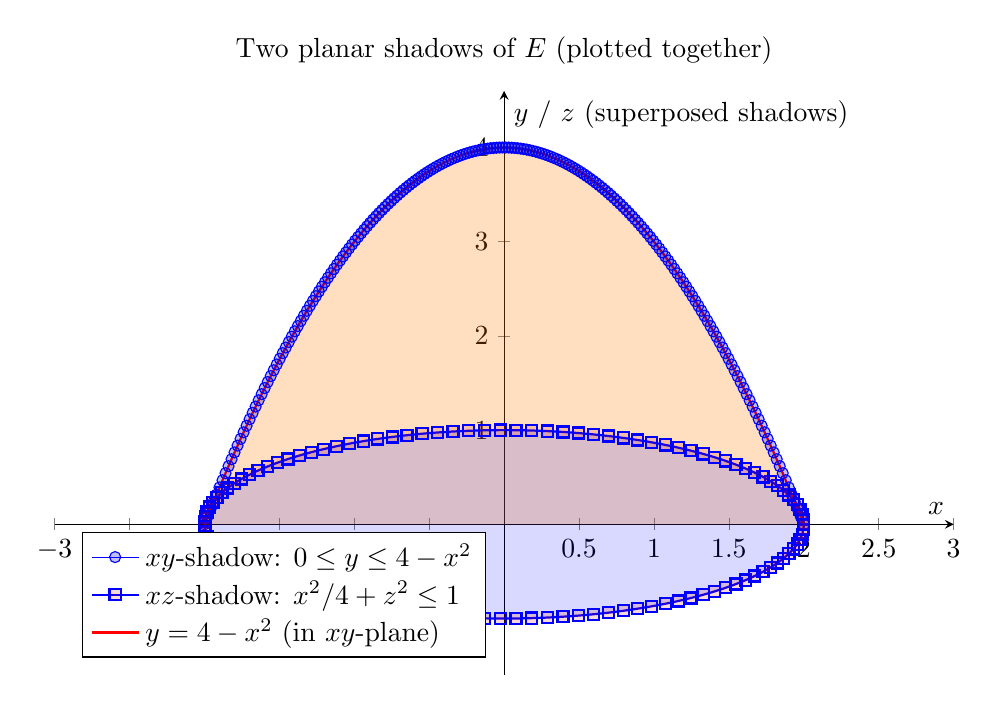
\begin{tikzpicture}
\begin{axis}[
    xlabel={$x$}, ylabel={$y$ / $z$ (superposed shadows)},
    title={Two planar shadows of $E$ (plotted together)},
    xmin=-3, xmax=3, ymin=-1.6, ymax=4.6,
    axis lines=middle,
    legend pos=south west, legend cell align=left,
    domain=-2:2, samples=200,
    width=13cm, height=9cm
]
% xy-shadow (parabola) filled
\addplot+[fill=orange, fill opacity=0.25, draw=none, domain=-2:2]
    {4-x^2} \closedcycle;
% xz-shadow (ellipse) filled
\addplot+[fill=blue, fill opacity=0.15, draw=blue, thick, domain=0:360, samples=120, smooth]
    ({2*cos(x)}, {sin(x)});
% parabola outline
\addplot[red, thick, domain=-2:2] {4-x^2};
\addlegendentry{$xy$-shadow: $0 \le y \le 4-x^2$}
\addlegendentry{$xz$-shadow: $x^2/4 + z^2 \le 1$}
\addlegendentry{$y = 4-x^2$ (in $xy$-plane)}
\end{axis}
\end{tikzpicture}
\end{document}